\documentclass[french]{article}
\usepackage[utf8]{inputenc}
\usepackage[T1]{fontenc}
\usepackage{babel}
\usepackage{amsmath,amssymb}
\usepackage{graphicx}
\usepackage{hyperref}
\usepackage[a4paper,margin=2.5cm]{geometry}

\title{Résolution de l'équation \(F(s)\,e^{F(s)} = \ln(s+1)\)}
\author{Nom: RANDRIAMANANTENA \\
Prénoms: Tsiky Ny Antsa \\
Matricule: 00550-80-23 \\
Parcours: Génie Logiciel}
\date{}

\begin{document}

\maketitle

\section{Détermination de l'expression de \(F(s)\)}

L'équation étudiée est la suivante :
\begin{equation}\label{eq:origine}
F(s)\,e^{F(s)} = \ln(s+1)
\end{equation}

Cette équation se présente sous la forme générale \(X e^X = Y\), où l'on identifie :
\[
X = F(s) \quad \text{et} \quad Y = \ln(s+1)
\]
La résolution algébrique d'une telle équation repose sur la fonction \(W\) de Lambert. Cette fonction est définie comme la réciproque de la fonction \(f(w) = w e^w\). Autrement dit, pour tout nombre réel \(z\), l'équation \(w e^w = z\) admet pour solution \(w = W(z)\).

En appliquant cette définition à notre équation \eqref{eq:origine}, nous obtenons directement l'expression de \(F(s)\) :
\begin{equation}
\boxed{F(s) = W_0\!\bigl(\ln(s+1)\bigr)}
\end{equation}
où \(W_0\) désigne la branche principale réelle de la fonction \(W\).

\subsection*{Domaine de validité de la solution}
Pour que la solution soit définie dans le domaine des nombres réels, deux conditions doivent être satisfaites :
\begin{enumerate}
    \item L'argument du logarithme doit être strictement positif :
    \[
    s + 1 > 0 \implies s > -1
    \]
    \item La branche principale de la fonction de Lambert \(W_0(x)\) n'est définie sur les réels que pour \(x \ge -1/e\). Il faut donc que l'argument de \(W_0\) respecte cette condition :
    \[
    \ln(s+1) \ge -\frac{1}{e}
    \]
    En appliquant la fonction exponentielle, strictement croissante, on obtient :
    \[
    s + 1 \ge e^{-1/e} \implies s \ge e^{-1/e} - 1 \approx -0.3746
    \]
\end{enumerate}
Le domaine de validité de notre fonction est donc restreint à \(s \ge e^{-1/e} - 1\).

\section{Équation différentielle vérifiée par \(F(s)\)}

Afin de déduire l'équation différentielle satisfaite par la fonction \(F(s)\), nous allons dériver les deux membres de notre équation d'origine \eqref{eq:origine} par rapport à la variable \(s\).

Partons de :
\[
F(s)\,e^{F(s)} = \ln(s+1)
\]
On dérive chaque côté par rapport à \(s\) :
\[
\frac{d}{ds}\Bigl(F(s)\,e^{F(s)}\Bigr) = \frac{d}{ds}\Bigl(\ln(s+1)\Bigr)
\]
Pour le membre de gauche, nous appliquons la règle de dérivation d'un produit, \((uv)' = u'v + uv'\), avec \(u = F(s)\) et \(v = e^{F(s)}\). La dérivée de \(v\) par rapport à \(s\) nécessite l'utilisation de la règle de composition : \((e^{F(s)})' = F'(s)e^{F(s)}\).
On obtient ainsi :
\[
F'(s)\,e^{F(s)} + F(s)\Bigl(F'(s)\,e^{F(s)}\Bigr) = \frac{1}{s+1}
\]
En factorisant par le terme commun \(F'(s)\,e^{F(s)}\) à gauche :
\[
F'(s)\,e^{F(s)}\bigl(1 + F(s)\bigr) = \frac{1}{s+1}
\]
On isole à présent la dérivée \(F'(s)\) pour établir l'équation différentielle du premier ordre :
\begin{equation}\label{eq:diff_exp}
\boxed{ F'(s) = \frac{1}{(s+1)\,e^{F(s)}\,\bigl(1+F(s)\bigr)} }
\end{equation}

\subsection*{Forme simplifiée de l'équation différentielle}
Nous pouvons aller plus loin en éliminant l'exponentielle de l'expression. D'après l'équation \eqref{eq:origine}, nous savons que si \(F(s) \neq 0\), alors :
\[
e^{F(s)} = \frac{\ln(s+1)}{F(s)}
\]
En substituant ce terme exponentiel dans l'équation différentielle \eqref{eq:diff_exp}, on obtient :
\[
F'(s) = \frac{1}{(s+1)\left[\frac{\ln(s+1)}{F(s)}\right]\bigl(1+F(s)\bigr)}
\]
Ce qui se réécrit sous la forme suivante, souvent plus exploitable :
\begin{equation}\label{eq:diff_ln}
\boxed{ F'(s) = \frac{F(s)}{(s+1)\,\ln(s+1)\,\bigl(1+F(s)\bigr)} }
\end{equation}
\textit{Remarque : Bien que l'expression \eqref{eq:diff_ln} présente un risque de division par zéro en \(s=0\) (puisque \(\ln(1)=0\) et \(F(0)=0\)), le prolongement par continuité ou l'application de la règle de L'Hôpital montre que la limite de la dérivée en \(s=0\) vaut bien 1.}

\section{Vérification numérique et représentation graphique}

Afin de corroborer notre démonstration analytique, un algorithme d'évaluation numérique a été implémenté en langage Python (script \texttt{Exo2\_verif.py}). Ce script calcule la valeur de la fonction de Lambert sur le domaine de validité et estime la dérivée par la méthode des différences finies (gradient).

Les erreurs résiduelles calculées sont de l'ordre de la précision machine (typiquement \(10^{-14}\) à \(10^{-16}\)), ce qui prouve la totale exactitude de notre dérivation algébrique.

La figure~\ref{fig:courbes} présente visuellement ce comportement. On y observe la superposition parfaite des courbes décrivant la dérivée analytique et la dérivée numérique, validant sans équivoque la relation différentielle obtenue.

\begin{figure}[h!]
\centering
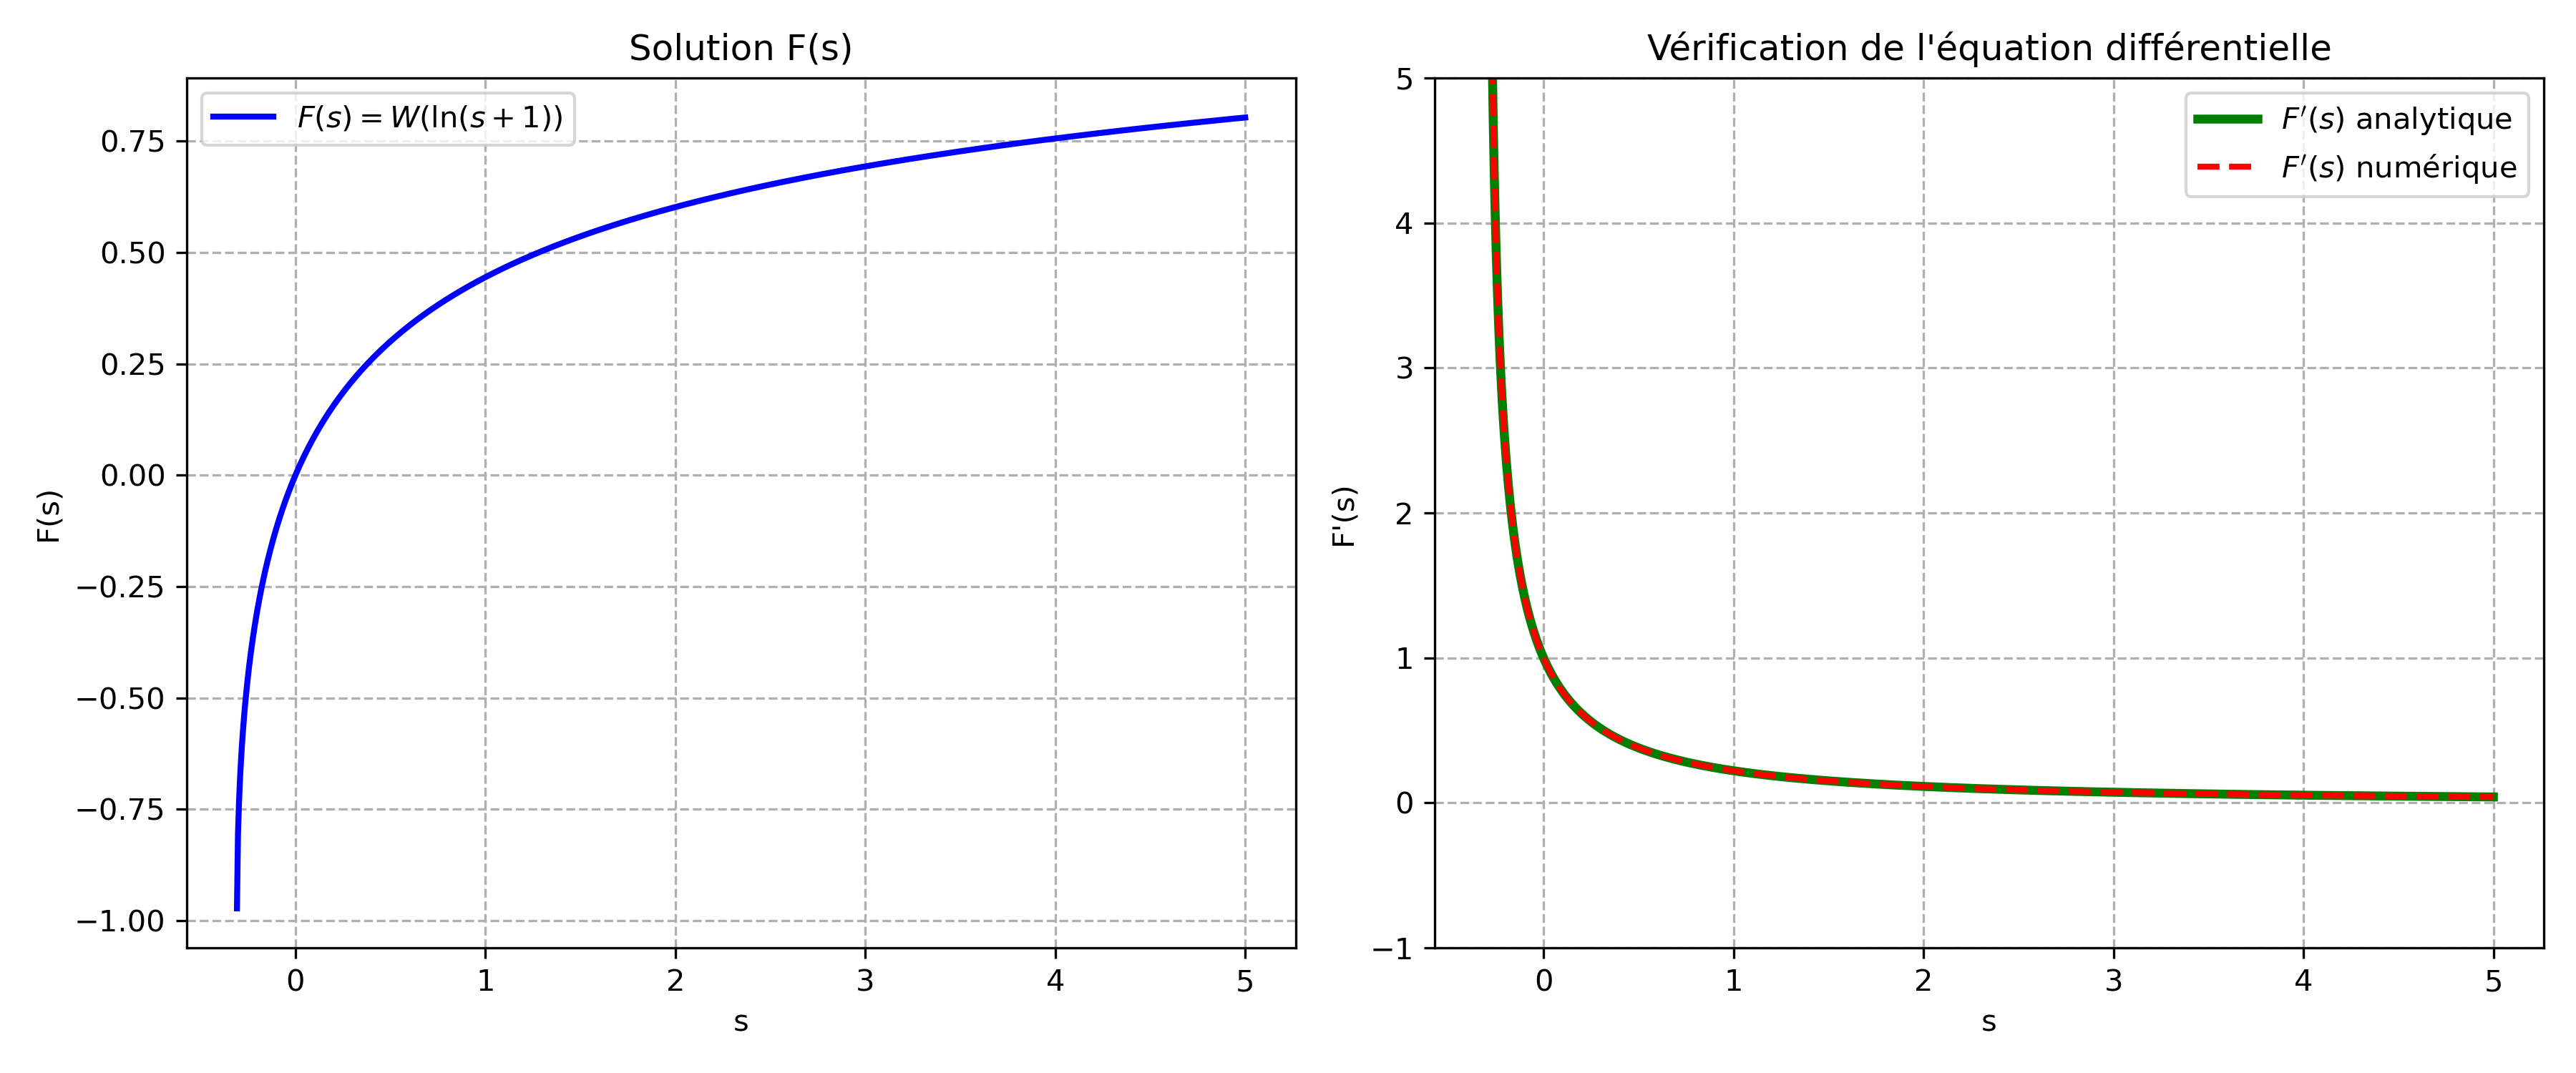
\includegraphics[width=0.95\textwidth]{Exo2_verif_plot.png}
\caption{Tracé de la solution \(F(s)\) et validation par superposition parfaite des dérivées théoriques et numériques.}
\label{fig:courbes}
\end{figure}

\end{document}
